\documentclass[10pt,aspectratio=169]{beamer}

\usetheme{Madrid}
\usecolortheme{default}
\setbeamertemplate{navigation symbols}{}

\usepackage{amsmath,amssymb}
\usepackage{array}
\usepackage{booktabs}
\usepackage{graphicx}
\usepackage{tikz}
\usepackage{xcolor}
\usetikzlibrary{positioning,arrows.meta,shapes.geometric,calc}

\title[Octopus RL Roadmap]{Octopus CXL Memory Pooling}
\subtitle{Systems evidence, current failure mode, and RL redesign roadmap}
\author{Pulak Mehrotra}
\date{March 2026}

\newcommand{\figorplaceholder}[2]{%
  \IfFileExists{#1}{%
    \includegraphics[width=\linewidth,height=#2,keepaspectratio]{#1}%
  }{%
    \fbox{\parbox[c][#2][c]{0.9\linewidth}{\centering Missing figure:\\\texttt{#1}}}%
  }%
}

\begin{document}

\begin{frame}
  \titlepage
\end{frame}

\begin{frame}{Roadmap}
  \tableofcontents
\end{frame}

\section{System Setting and Current Failure}

% Sources:
% - context/rl_memory_pooling_roadmap_v2.md §§1, 2, 3
% - context/cluade-convo-summary.md §§4, 5, 6, 7, 9
% - octopus-allocation/docs/overview/v1/v1.tex
\begin{frame}{Problem Setting}
  \begin{columns}[T,onlytextwidth]
    \column{0.55\textwidth}
      \centering
      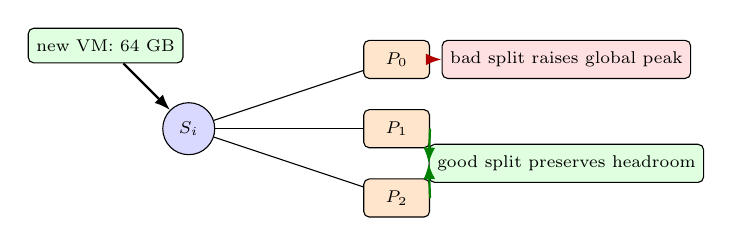
\begin{tikzpicture}[
          scale=0.88,
          transform shape,
          every node/.style={font=\scriptsize},
          host/.style={draw, circle, fill=blue!15, minimum size=0.75cm},
          mpd/.style={draw, rectangle, rounded corners=2pt, fill=orange!20, minimum width=0.95cm, minimum height=0.55cm},
          note/.style={draw, rounded corners=2pt, fill=green!12, minimum width=1.55cm, minimum height=0.5cm},
          good/.style={draw, rounded corners=2pt, fill=green!12, minimum width=2.5cm, minimum height=0.55cm},
          bad/.style={draw, rounded corners=2pt, fill=red!12, minimum width=2.5cm, minimum height=0.55cm}
      ]
        \node[host] (h) at (0,0) {$S_i$};
        \node[note] (vm) at (-1.2,1.2) {new VM: 64 GB};
        \node[mpd] (p0) at (3.0,1.0) {$P_0$};
        \node[mpd] (p1) at (3.0,0.0) {$P_1$};
        \node[mpd] (p2) at (3.0,-1.0) {$P_2$};
        \draw[-{Latex[length=2mm]}, thick] (vm) -- (h);
        \draw (h) -- (p0);
        \draw (h) -- (p1);
        \draw (h) -- (p2);
        \node[bad] (bad) at (5.45,1.0) {bad split raises global peak};
        \node[good] (good) at (5.45,-0.5) {good split preserves headroom};
        \draw[-{Latex[length=2mm]}, thick, red!70!black] (p0.east) -- (bad.west);
        \draw[-{Latex[length=2mm]}, thick, green!50!black] (p1.east) -- (good.west);
        \draw[-{Latex[length=2mm]}, thick, green!50!black] (p2.east) -- (good.west);
      \end{tikzpicture}
    \column{0.45\textwidth}
      \begin{itemize}
        \item Each VM arrival triggers one memory-allocation decision.
        \item A host can only use its physically connected MPDs.
        \item There is no cheap migration loop to fix bad placements later.
        \item We care about the worst MPD peak because every MPD must be provisioned to survive it.
      \end{itemize}
  \end{columns}

  \vspace{0.7em}
  {\small
  \begin{equation*}
    \text{Current savings} = 1 -
    \frac{m \cdot \max_{j}\{\text{PeakLoad}_{j}\}}
         {\text{total pod DRAM}}
  \end{equation*}
  }
\end{frame}

\begin{frame}{Octopus Topology Makes Allocation Hard}
  \begin{columns}[T,onlytextwidth]
    \column{0.52\textwidth}
      \centering
      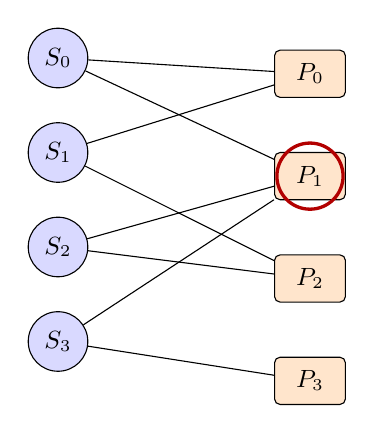
\begin{tikzpicture}[
          every node/.style={font=\small},
          host/.style={draw, circle, fill=blue!15, minimum size=0.65cm},
          mpd/.style={draw, rectangle, rounded corners=2pt, fill=orange!20, minimum height=0.6cm, minimum width=0.9cm}
      ]
        \node[host] (h0) at (0,2.2) {$S_0$};
        \node[host] (h1) at (0,1.0) {$S_1$};
        \node[host] (h2) at (0,-0.2) {$S_2$};
        \node[host] (h3) at (0,-1.4) {$S_3$};

        \node[mpd] (p0) at (3.2,2.0) {$P_0$};
        \node[mpd] (p1) at (3.2,0.7) {$P_1$};
        \node[mpd] (p2) at (3.2,-0.6) {$P_2$};
        \node[mpd] (p3) at (3.2,-1.9) {$P_3$};

        \draw (h0) -- (p0);
        \draw (h0) -- (p1);
        \draw (h1) -- (p0);
        \draw (h1) -- (p2);
        \draw (h2) -- (p1);
        \draw (h2) -- (p2);
        \draw (h3) -- (p1);
        \draw (h3) -- (p3);

        \draw[red!70!black, very thick] (p1) circle (0.42);
      \end{tikzpicture}
    \column{0.48\textwidth}
      \begin{itemize}
        \item Servers and MPDs form a sparse bipartite graph, not a fully connected pool.
        \item A hot subset of servers can collide on the same small MPD neighborhood.
        \item A choice that looks good for one server can still overload a shared MPD later.
        \item So Octopus is harder than ``just spread load evenly''.
      \end{itemize}

      \vspace{0.4em}
      \textbf{Systems takeaway:} topology is part of the problem statement, not a detail of the simulator.
  \end{columns}
\end{frame}

% Sources:
% - octopus-allocation/docs/overview/v1/slides/slides_rl_octopus.tex
% - context/cluade-convo-summary.md §4.4
\begin{frame}{Why Pooling Helps}
  \begin{columns}[T,onlytextwidth]
    \column{0.63\textwidth}
      \figorplaceholder{../octopus-allocation/docs/overview/v1/figs/peak_to_mean.pdf}{0.67\textheight}
    \column{0.37\textwidth}
      \begin{itemize}
        \item Azure traces across \textbf{10 datacenters} show unsynchronized peaks.
        \item Cluster peak-to-mean ratio is about \textbf{1.13--1.26x}.
        \item That gap is exactly the headroom memory pooling tries to recover.
        \item The pooling opportunity is real before we even talk about RL.
      \end{itemize}
  \end{columns}
\end{frame}

% \begin{frame}{Existing Project Evidence Before RL}
%   \begin{columns}[T,onlytextwidth]
%     \column{0.5\textwidth}
%       \begin{block}{Existing project evidence}
%         \begin{itemize}
%           \item Break-even is only about \textbf{3\%} pooling savings.
%           \item Prior Octopus analysis reports about \textbf{16\%} greedy savings on Acadia-96.
%           \item Fully connected memory pooling is the upper benchmark.
%           \item The greedy-to-optimal gap is what a better learned allocator should close.
%         \end{itemize}
%       \end{block}
%     \column{0.5\textwidth}
%       \centering
%       \begin{tikzpicture}[
%           x=1cm, y=1cm,
%           bar/.style={draw, fill=blue!18, minimum width=1.4cm, align=center, font=\scriptsize},
%           axislabel/.style={font=\scriptsize}
%       ]
%         \draw[->] (0,0) -- (0,4.2);
%         \draw[->] (0,0) -- (5.5,0);
%         \node[axislabel, rotate=90] at (-0.55,2.1) {savings};
%         \node[bar, minimum height=0.45cm] at (1.2,0.25) {break-even\\3\%};
%         \node[bar, minimum height=2.3cm, fill=green!20] at (3.3,1.15) {greedy\\16\%};
%         \node[bar, minimum height=2.8cm, fill=orange!20] at (4.8,1.40) {upper bound\\higher};
%         \draw[dashed] (0,0.45) -- (5.2,0.45);
%       \end{tikzpicture}
%
%       \vspace{0.5em}
%       {\scriptsize Existing project evidence from prior Octopus analysis, not newly regenerated in this checkout.}
%   \end{columns}
% \end{frame}

\begin{frame}{Current Implementation}
  \begin{columns}[T,onlytextwidth]
    \column{0.54\textwidth}
      \centering
      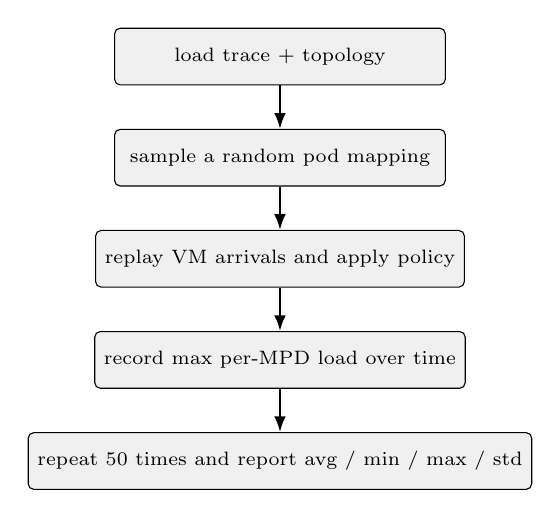
\begin{tikzpicture}[
          node distance=0.55cm,
          box/.style={draw, rounded corners=2pt, minimum width=4.2cm, minimum height=0.72cm, align=center, fill=black!6, font=\scriptsize},
          arr/.style={-{Latex[length=2mm]}, thick}
      ]
        \node[box] (trace) {load trace + topology};
        \node[box, below=of trace] (map) {sample a random pod mapping};
        \node[box, below=of map] (sim) {replay VM arrivals and apply policy};
        \node[box, below=of sim] (peak) {record max per-MPD load over time};
        \node[box, below=of peak] (agg) {repeat 50 times and report avg / min / max / std};
        \draw[arr] (trace) -- (map);
        \draw[arr] (map) -- (sim);
        \draw[arr] (sim) -- (peak);
        \draw[arr] (peak) -- (agg);
      \end{tikzpicture}
    \column{0.46\textwidth}
      \begin{itemize}
        \item `evaluate.py` does not score one cherry-picked topology.
        \item It repeats evaluation over many random pod mappings.
        \item The reported number is a distribution of pooling savings, not one run.
        \item This is a systems metric: required per-MPD capacity under trace replay.
      \end{itemize}
  \end{columns}
\end{frame}

\begin{frame}{Why Current SAC Fails Right Now}
  \begin{columns}[T,onlytextwidth]
    \column{0.48\textwidth}
      \centering
      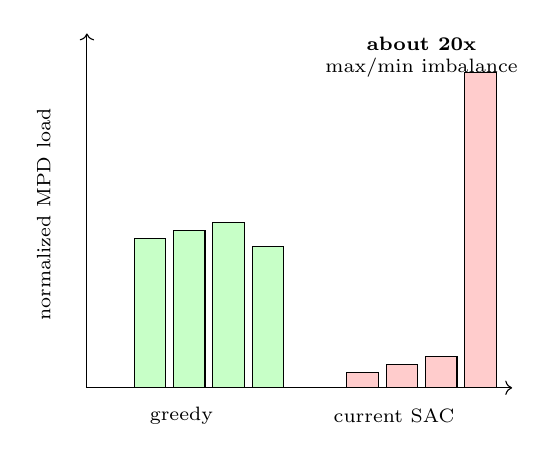
\begin{tikzpicture}[
          x=1cm, y=1cm,
          lbl/.style={font=\scriptsize},
          bar1/.style={draw, fill=green!22},
          bar2/.style={draw, fill=red!20}
      ]
        \draw[->] (0,0) -- (0,4.5);
        \draw[->] (0,0) -- (5.4,0);
        \node[lbl, rotate=90] at (-0.55,2.2) {normalized MPD load};
        \node[lbl] at (1.2,-0.35) {greedy};
        \node[lbl] at (3.9,-0.35) {current SAC};
        \draw[bar1] (0.6,0) rectangle (1.0,1.9);
        \draw[bar1] (1.1,0) rectangle (1.5,2.0);
        \draw[bar1] (1.6,0) rectangle (2.0,2.1);
        \draw[bar1] (2.1,0) rectangle (2.5,1.8);
        \draw[bar2] (3.3,0) rectangle (3.7,0.2);
        \draw[bar2] (3.8,0) rectangle (4.2,0.3);
        \draw[bar2] (4.3,0) rectangle (4.7,0.4);
        \draw[bar2] (4.8,0) rectangle (5.2,4.0);
        \node[lbl, align=center] at (4.25,4.2) {\textbf{about 20x}\\max/min imbalance};
      \end{tikzpicture}
    \column{0.52\textwidth}
      \begin{itemize}
        \item Current agent: \textbf{SAC}, 1M steps, fast configuration.
        \item The failure is behavioral: load collapses onto a few MPDs.
        \item Diagnostics point to:
          \begin{itemize}
            \item sparse reward
            \item missing future-pressure features
            \item missing temporal features
            \item too little training
            \item weak train/eval diversification
          \end{itemize}
        \item This is a \textbf{learnability problem} first, not a forgetting problem yet.
      \end{itemize}
  \end{columns}
\end{frame}

\begin{frame}{Training-Time Learnability vs Deployment-Time Forgetting}
  \centering
  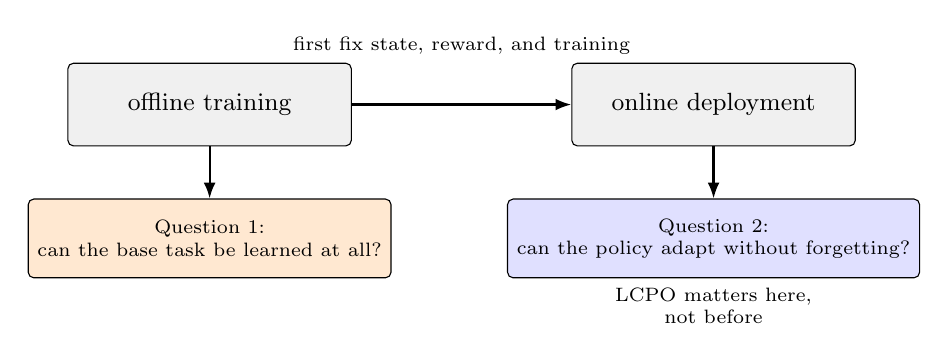
\begin{tikzpicture}[
      x=1cm, y=1cm,
      stage/.style={draw, rounded corners=2pt, minimum width=3.6cm, minimum height=1.05cm, align=center, font=\small, fill=black!6},
      note/.style={draw, rounded corners=2pt, minimum width=4.2cm, minimum height=1.0cm, align=center, font=\scriptsize},
      arr/.style={-{Latex[length=2mm]}, thick}
  ]
    \node[stage] (offline) at (2.3,2.4) {offline training};
    \node[stage] (deploy) at (8.7,2.4) {online deployment};
    \node[note, fill=orange!18] (learn) at (2.3,0.7) {Question 1:\\can the base task be learned at all?};
    \node[note, fill=blue!12] (forget) at (8.7,0.7) {Question 2:\\can the policy adapt without forgetting?};
    \draw[arr] (offline) -- (deploy);
    \draw[arr] (offline) -- (learn);
    \draw[arr] (deploy) -- (forget);
    \node[font=\scriptsize, align=center] at (5.5,3.15) {first fix state, reward, and training};
    \node[font=\scriptsize, align=center] at (8.7,-0.15) {LCPO matters here,\\not before};
  \end{tikzpicture}
\end{frame}

\begin{frame}{Redesign Roadmap}
  \centering
  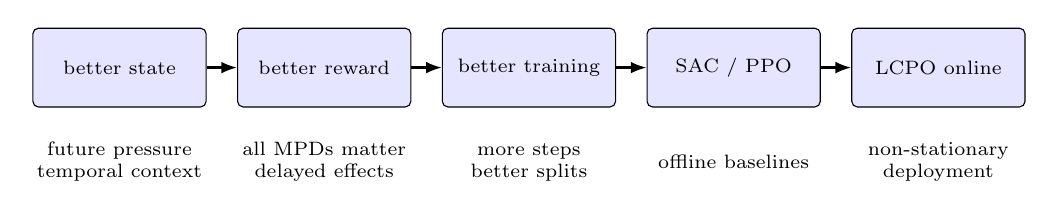
\begin{tikzpicture}[
      x=1cm, y=1cm,
      roadstep/.style={draw, rounded corners=2pt, minimum width=2.2cm, minimum height=1.0cm, align=center, font=\scriptsize, fill=blue!10},
      arr/.style={-{Latex[length=2mm]}, thick}
  ]
    \node[roadstep] (s1) at (1.4,1.4) {better state};
    \node[roadstep] (s2) at (4.0,1.4) {better reward};
    \node[roadstep] (s3) at (6.6,1.4) {better training};
    \node[roadstep] (s4) at (9.2,1.4) {SAC / PPO};
    \node[roadstep] (s5) at (11.8,1.4) {LCPO online};
    \draw[arr] (s1) -- (s2);
    \draw[arr] (s2) -- (s3);
    \draw[arr] (s3) -- (s4);
    \draw[arr] (s4) -- (s5);
    \node[font=\scriptsize, align=center] at (1.4,0.2) {future pressure\\temporal context};
    \node[font=\scriptsize, align=center] at (4.0,0.2) {all MPDs matter\\delayed effects};
    \node[font=\scriptsize, align=center] at (6.6,0.2) {more steps\\better splits};
    \node[font=\scriptsize, align=center] at (9.2,0.2) {offline baselines};
    \node[font=\scriptsize, align=center] at (11.8,0.2) {non-stationary\\deployment};
  \end{tikzpicture}

  \vspace{0.7em}
  \textbf{Main message:} first make the task learnable, then solve online forgetting.
\end{frame}

\section{State Redesign}

% Sources:
% - octopus-allocation/octopus/env.py
% - octopus-allocation/scripts/train.py
\begin{frame}{Current Decision Pipeline in the Code}
  \centering
  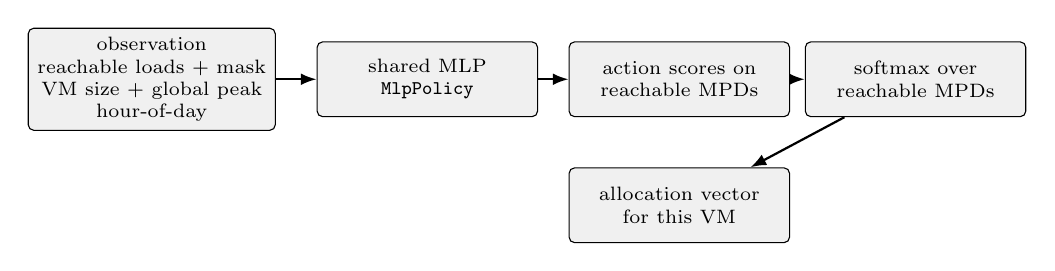
\begin{tikzpicture}[
      x=1cm, y=1cm,
      box/.style={draw, rounded corners=2pt, minimum width=2.8cm, minimum height=0.95cm, align=center, font=\scriptsize, fill=black!6},
      arr/.style={-{Latex[length=2mm]}, thick}
  ]
    \node[box] (obs) at (1.7,1.8) {observation\\reachable loads + mask\\VM size + global peak\\hour-of-day};
    \node[box] (mlp) at (5.2,1.8) {shared MLP\\\texttt{MlpPolicy}};
    \node[box] (logits) at (8.4,1.8) {action scores on\\reachable MPDs};
    \node[box] (softmax) at (11.4,1.8) {softmax over\\reachable MPDs};
    \node[box] (alloc) at (8.4,0.2) {allocation vector\\for this VM};
    \draw[arr] (obs) -- (mlp);
    \draw[arr] (mlp) -- (logits);
    \draw[arr] (logits) -- (softmax);
    \draw[arr] (softmax) -- (alloc);
  \end{tikzpicture}

  \vspace{0.5em}
  \begin{itemize}
    \item The model \emph{does} see each reachable MPD separately.
    \item It still does not see how each MPD is likely to fill up over time.
    \item The problem is not missing MPD slots in the input.
    \item The real issue is that the current state is too instantaneous and the reward is too sparse.
  \end{itemize}
\end{frame}

% Sources:
% - context/rl_memory_pooling_roadmap_v2.md §2.1-2.4
% - context/cluade-convo-summary.md §6
\begin{frame}{State Space Redesign: Adding More MPD Data}
  \begin{columns}[T,onlytextwidth]
    \column{0.52\textwidth}
      \centering
      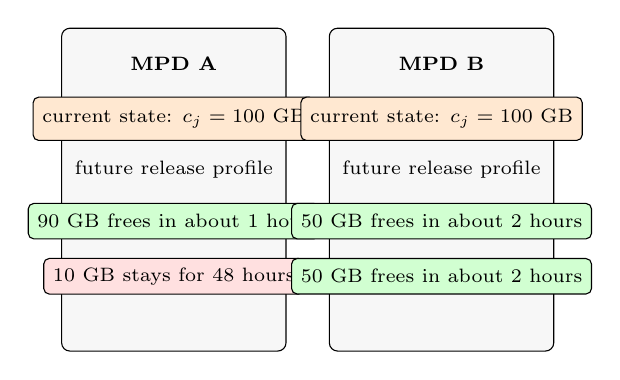
\begin{tikzpicture}[
          x=1cm, y=1cm,
          every node/.style={font=\scriptsize},
          panel/.style={draw, rounded corners=3pt, minimum width=2.85cm, minimum height=4.1cm, fill=black!3},
          cur/.style={draw, rounded corners=2pt, minimum width=2.2cm, minimum height=0.55cm, fill=orange!18},
          soon/.style={draw, rounded corners=2pt, minimum width=2.1cm, minimum height=0.45cm, fill=green!18},
          stick/.style={draw, rounded corners=2pt, minimum width=2.1cm, minimum height=0.45cm, fill=red!12},
          lbl/.style={font=\scriptsize, align=center}
      ]
        \node[panel] (a) at (-1.7,0.1) {};
        \node[lbl] at (-1.7,1.7) {\textbf{MPD A}};
        \node[cur] at (-1.7,1.0) {current state: $c_j = 100$ GB};
        \node[lbl] at (-1.7,0.35) {future release profile};
        \node[soon] at (-1.7,-0.3) {$90$ GB frees in about 1 hour};
        \node[stick] at (-1.7,-1.0) {$10$ GB stays for 48 hours};

        \node[panel] (b) at (1.7,0.1) {};
        \node[lbl] at (1.7,1.7) {\textbf{MPD B}};
        \node[cur] at (1.7,1.0) {current state: $c_j = 100$ GB};
        \node[lbl] at (1.7,0.35) {future release profile};
        \node[soon] at (1.7,-0.3) {$50$ GB frees in about 2 hours};
        \node[soon] at (1.7,-1.0) {$50$ GB frees in about 2 hours};
      \end{tikzpicture}
    \column{0.48\textwidth}
      \begin{itemize}
        \item Current state keeps only one scalar per MPD: $c_j =$ current load.
        \item So MPD A and MPD B both collapse to the same observed value, $c_j = 100$ GB.
        \item But their future headroom is very different.
        \item Add per-MPD features for:
          \begin{itemize}
            \item short-term release within 1 hour
            \item medium-term release within 4 hours
            \item sticky load weighted by remaining lifetime
            \item VM count as a fragmentation signal
          \end{itemize}
        \item VM lifetime is estimatable at arrival, so these features are computable.
      \end{itemize}
  \end{columns}

  \vspace{0.25em}
  {\scriptsize
  Sticky load alone is useful, but not sufficient: it tells us how locked an MPD is overall, while the release-horizon features tell us \textbf{when} capacity comes back.

  \vspace{0.2em}
  Citation: Pond (ASPLOS 2023), \href{https://pages.cs.wisc.edu/~markhill/papers/asplos2023_pond.pdf}{paper link}}
\end{frame}

\begin{frame}{State Space Redesign: Adding Temporal Data}
  \begin{columns}[T,onlytextwidth]
    \column{0.56\textwidth}
      \small
      \begin{tabular}{p{0.35\linewidth}p{0.56\linewidth}}
        \toprule
        \textbf{Temporal feature} & \textbf{What it adds} \\
        \midrule
        Per-MPD deltas & Whether each MPD is filling or draining \\
        Per-server deltas & Whether local pressure is ramping up \\
        Recent SLO summaries & Whether congestion is getting worse \\
        Hour-of-day context & Where we are in the diurnal cycle \\
        \bottomrule
      \end{tabular}
    \column{0.44\textwidth}
      \begin{itemize}
        \item The current policy mostly sees position, not velocity.
        \item Two MPDs with the same current load can have opposite near-future trends.
        \item Temporal features tell the policy whether pressure is rising, stable, or falling.
        \item Systems intuition: if traces are diurnal, timing information is operationally valuable.
      \end{itemize}
  \end{columns}
\end{frame}

\begin{frame}{Why We Need More Than One New MPD Feature}
  \begin{columns}[T,onlytextwidth]
    \column{0.56\textwidth}
      \small
      \begin{tabular}{p{0.35\linewidth}p{0.56\linewidth}}
        \toprule
        \textbf{Feature} & \textbf{What it adds} \\
        \midrule
        Short release & Near-term memory that opens up \\
        Medium release & Headroom that appears a bit later \\
        Sticky load & How trapped the MPD is overall \\
        VM count & Concentrated vs fragmented occupancy \\
        \bottomrule
      \end{tabular}
    \column{0.44\textwidth}
      \begin{itemize}
        \item Sticky load is one summary, not the whole story.
        \item Release-horizon features preserve timing.
        \item VM count captures fragmentation that total load can miss.
        \item The policy needs \textbf{how much}, \textbf{how soon}, and \textbf{how fragmented}.
      \end{itemize}
  \end{columns}
\end{frame}

\section{Reward Redesign}

% Sources:
% - octopus-allocation/octopus/env.py
% - context/rl_memory_pooling_roadmap_v2.md §3
% - context/cluade-convo-summary.md §7
\begin{frame}{Why Peak-Only Reward Ignores Most MPDs}
  \begin{columns}[T,onlytextwidth]
    \column{0.5\textwidth}
      \centering
      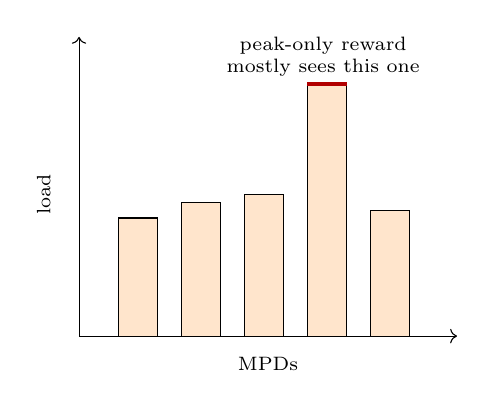
\begin{tikzpicture}[
          x=1cm, y=1cm,
          bar/.style={draw, fill=orange!20},
          lbl/.style={font=\scriptsize}
      ]
        \draw[->] (0,0) -- (0,3.8);
        \draw[->] (0,0) -- (4.8,0);
        \draw[bar] (0.5,0) rectangle (1.0,1.5);
        \draw[bar] (1.3,0) rectangle (1.8,1.7);
        \draw[bar] (2.1,0) rectangle (2.6,1.8);
        \draw[bar] (2.9,0) rectangle (3.4,3.2);
        \draw[bar] (3.7,0) rectangle (4.2,1.6);
        \draw[red!70!black, very thick] (2.9,3.2) -- (3.4,3.2);
        \node[lbl, align=center] at (2.4,-0.35) {MPDs};
        \node[lbl, rotate=90] at (-0.45,1.8) {load};
        \node[lbl, align=center] at (3.1,3.55) {peak-only reward\\mostly sees this one};
      \end{tikzpicture}
    \column{0.5\textwidth}
      \begin{itemize}
        \item Current reward changes only when the global peak changes.
        \item If action quality differs among non-peak MPDs, reward can stay unchanged.
        \item So the network sees all MPDs, but the scalar reward mostly scores one of them.
        \item Result: the policy can ignore most of the load-distribution structure.
      \end{itemize}

      \vspace{0.5em}
      \begin{equation*}
        r_t = -\frac{\text{peak}_{\text{after}} - \text{peak}_{\text{before}}}{\text{fairShare}}
      \end{equation*}
  \end{columns}
\end{frame}

\begin{frame}{Reward Redesign: New Immediate Reward}
  \begin{columns}[T,onlytextwidth]
    \column{0.44\textwidth}
      \begin{block}{Old immediate reward}
        \begin{itemize}
          \item mostly controls the current worst MPD
          \item sparse signal
          \item weak incentive to spread load
        \end{itemize}
      \end{block}
      \begin{block}{New immediate reward}
        \begin{itemize}
          \item peak penalty
          \item variance penalty
          \item oversubscribed-MPD penalty
        \end{itemize}
      \end{block}
    \column{0.56\textwidth}
      {\small
      \begin{equation*}
        R_t
        = \alpha \cdot \text{PeakTerm}(t)
        - \beta \cdot \text{VarianceTerm}(t)
        - \gamma \cdot \text{OverCapMPD}(t)
      \end{equation*}
      \begin{equation*}
        \text{PeakTerm}(t) = 1 - \frac{\max_j\{c_j(t)\}}{\text{cap}_{\max}}
      \end{equation*}
      \begin{equation*}
        \text{VarianceTerm}(t) = \mathrm{Var}(c(t))
      \end{equation*}
      \begin{equation*}
        \text{OverCapMPD}(t) = \sum_j \max\{0,\, c_j(t) - \text{cap}_j\}
      \end{equation*}
      }

      \begin{itemize}
        \item This is easier to optimize than peak-only reward because all three terms move during training.
        \item The oversubscribed-MPD term is a direct penalty on capacity violations, not a generic ``SLO'' abstraction.
      \end{itemize}
  \end{columns}
\end{frame}

\begin{frame}{Reward Redesign: Why Each Term Matters}
  \begin{columns}[T,onlytextwidth]
    \column{0.58\textwidth}
      \small
      \begin{tabular}{p{0.24\linewidth}p{0.30\linewidth}p{0.36\linewidth}}
        \toprule
        \textbf{Term} & \textbf{What it measures} & \textbf{Why we need it} \\
        \midrule
        Peak term & current worst MPD load & keeps the reward aligned with the true capacity objective \\
        Variance term & imbalance across MPDs & gives dense feedback so non-peak MPDs matter too \\
        Over-cap term & total oversubscribed memory across MPDs & makes capacity violations a hard penalty rather than an afterthought \\
        \bottomrule
      \end{tabular}
    \column{0.42\textwidth}
      \begin{itemize}
        \item \textbf{Peak term only} is not enough:
          \begin{itemize}
            \item it mostly watches one MPD
            \item it can ignore imbalance elsewhere
          \end{itemize}
        \item \textbf{Variance term only} is not enough:
          \begin{itemize}
            \item perfectly balanced but very high load is still bad
          \end{itemize}
        \item \textbf{Over-cap term} matters because oversubscription is the real operational failure mode.
        \item Together the reward pushes toward \textbf{uniformly low} load, not merely balanced load.
      \end{itemize}
  \end{columns}
\end{frame}

\begin{frame}{Reward Redesign: Post-Termination Credit}
  \begin{columns}[T,onlytextwidth]
    \column{0.56\textwidth}
      \centering
      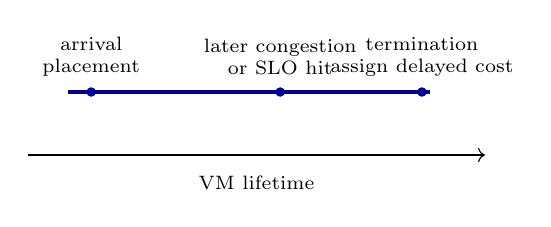
\begin{tikzpicture}[
          x=1cm, y=1cm,
          lbl/.style={font=\scriptsize},
          arr/.style={-{Latex[length=2mm]}, thick}
      ]
        \draw[->] (0,0) -- (5.8,0);
        \node[lbl] at (2.9,-0.35) {VM lifetime};
        \draw[very thick, blue!60!black] (0.5,0.8) -- (5.1,0.8);
        \filldraw[blue!60!black] (0.8,0.8) circle (1.5pt);
        \filldraw[blue!60!black] (3.2,0.8) circle (1.5pt);
        \filldraw[blue!60!black] (5.0,0.8) circle (1.5pt);
        \node[lbl, align=center] at (0.8,1.25) {arrival\\placement};
        \node[lbl, align=center] at (3.2,1.25) {later congestion\\or SLO hit};
        \node[lbl, align=center] at (5.0,1.25) {termination\\assign delayed cost};
      \end{tikzpicture}
    \column{0.44\textwidth}
      \begin{itemize}
        \item A bad placement can look harmless immediately.
        \item The real damage may appear hours later when later VMs arrive.
        \item Add a termination-time reward for:
          \begin{itemize}
            \item lifetime SLO impact
            \item migration cost if migration is ever allowed
          \end{itemize}
        \item This is how we address long-horizon credit assignment.
      \end{itemize}
  \end{columns}
\end{frame}

\section{Training and Data}

% Sources:
% - octopus-allocation/scripts/train.py
% - octopus-allocation/scripts/evaluate.py
\begin{frame}{Current Octopus Training and Evaluation Pipeline}
  \begin{columns}[T,onlytextwidth]
    \column{0.56\textwidth}
      \centering
      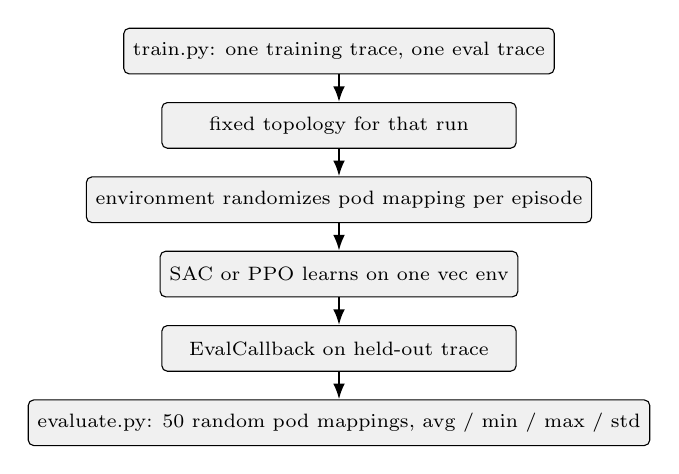
\begin{tikzpicture}[
          node distance=0.35cm,
          box/.style={draw, rounded corners=2pt, minimum width=4.5cm, minimum height=0.58cm, align=center, font=\scriptsize, fill=black!6},
          arr/.style={-{Latex[length=2mm]}, thick}
      ]
        \node[box] (trace) {train.py: one training trace, one eval trace};
        \node[box, below=of trace] (topo) {fixed topology for that run};
        \node[box, below=of topo] (env) {environment randomizes pod mapping per episode};
        \node[box, below=of env] (model) {SAC or PPO learns on one vec env};
        \node[box, below=of model] (eval) {EvalCallback on held-out trace};
        \node[box, below=of eval] (post) {evaluate.py: 50 random pod mappings, avg / min / max / std};
        \draw[arr] (trace) -- (topo);
        \draw[arr] (topo) -- (env);
        \draw[arr] (env) -- (model);
        \draw[arr] (model) -- (eval);
        \draw[arr] (eval) -- (post);
      \end{tikzpicture}
    \column{0.44\textwidth}
      \begin{itemize}
        \item Current code path is simple and reproducible.
        \item It already has some randomness through pod assignment.
        \item But it is still one-trace, one-topology training per run.
        \item There is no curriculum yet.
      \end{itemize}
  \end{columns}
  \vspace{0.2em}
  {\tiny Sources: \texttt{octopus-allocation/scripts/train.py}, \texttt{octopus-allocation/scripts/evaluate.py}}
\end{frame}

\begin{frame}{What Is Curriculum Learning?}
  \begin{columns}[T,onlytextwidth]
    \column{0.54\textwidth}
      \centering
      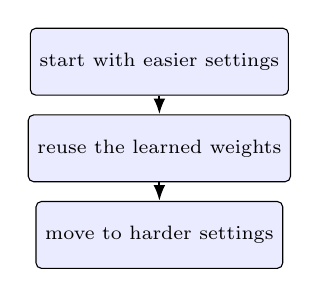
\begin{tikzpicture}[
          x=1cm, y=1cm,
          stage/.style={draw, rounded corners=2pt, minimum width=2.8cm, minimum height=0.85cm, align=center, font=\scriptsize, fill=blue!8},
          arr/.style={-{Latex[length=2mm]}, thick}
      ]
        \node[stage] (s1) at (1.7,2.2) {start with easier settings};
        \node[stage] (s2) at (1.7,1.1) {reuse the learned weights};
        \node[stage] (s3) at (1.7,0.0) {move to harder settings};
        \draw[arr] (s1) -- (s2);
        \draw[arr] (s2) -- (s3);
      \end{tikzpicture}
    \column{0.46\textwidth}
      \begin{itemize}
        \item Curriculum learning means \textbf{training in stages}, not jumping directly to the hardest setting.
        \item Each stage teaches a simpler version of the same task.
        \item The model carries its weights forward as the task gets harder.
        \item Goal: learn the balancing pattern first, then learn large-scale generalization.
      \end{itemize}
  \end{columns}
  \vspace{0.2em}
  {\tiny Sources: roadmap notes and conversation summary in the slide context folder}
\end{frame}

\begin{frame}{Current Pipeline vs Proposed Curriculum}
  \centering
  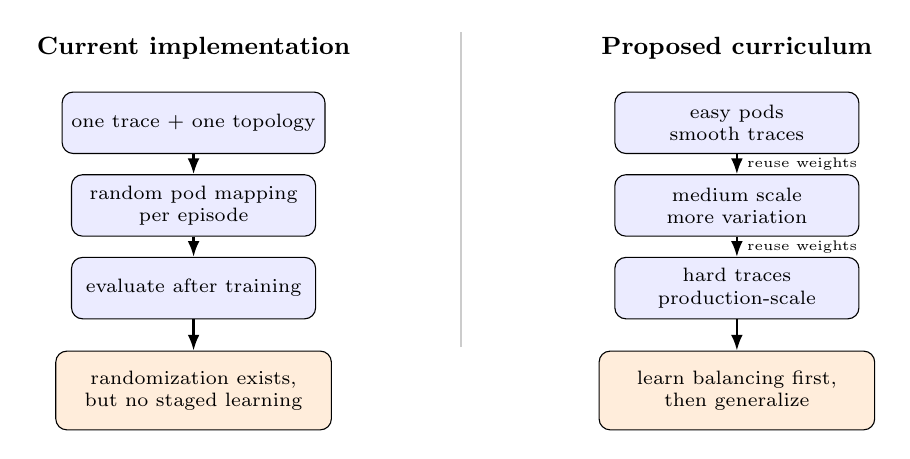
\begin{tikzpicture}[
    x=1cm, y=1cm,
    stage/.style={
      draw,
      rounded corners,
      align=center,
      minimum width=3.1cm,
      minimum height=0.78cm,
      fill=blue!8,
      font=\scriptsize
    },
    outcome/.style={
      draw,
      rounded corners,
      align=center,
      minimum width=3.5cm,
      minimum height=1.0cm,
      fill=orange!14,
      font=\scriptsize
    },
    arrow/.style={-{Latex[length=2mm]}, thick}
  ]
    \draw[gray!40, line width=0.3mm] (6.5,0.2) -- (6.5,4.2);

    \node[font=\small\bfseries] at (3.1, 4.0) {Current implementation};
    \node[stage] (c1) at (3.1, 3.05) {one trace + one topology};
    \node[stage] (c2) at (3.1, 2.0) {random pod mapping\\per episode};
    \node[stage] (c3) at (3.1, 0.95) {evaluate after training};
    \draw[arrow] (c1) -- (c2);
    \draw[arrow] (c2) -- (c3);
    \node[outcome] (co) at (3.1, -0.35) {randomization exists,\\but no staged learning};
    \draw[arrow] (c3.south) -- (co.north);

    \node[font=\small\bfseries] at (10.0, 4.0) {Proposed curriculum};
    \node[stage] (p1) at (10.0, 3.05) {easy pods\\smooth traces};
    \node[stage] (p2) at (10.0, 2.0) {medium scale\\more variation};
    \node[stage] (p3) at (10.0, 0.95) {hard traces\\production-scale};
    \draw[arrow] (p1) -- node[right,font=\tiny] {reuse weights} (p2);
    \draw[arrow] (p2) -- node[right,font=\tiny] {reuse weights} (p3);
    \node[outcome] (po) at (10.0, -0.35) {learn balancing first,\\then generalize};
    \draw[arrow] (p3.south) -- (po.north);
  \end{tikzpicture}
  \vspace{0.2em}

  {\tiny Left: current code path from \texttt{train.py} and \texttt{evaluate.py}. Right: proposed staged training from the roadmap/context notes.}
\end{frame}

\begin{frame}{Domain Randomization and Train/Eval Split}
  \begin{columns}[T,onlytextwidth]
    \column{0.56\textwidth}
      \small
      \begin{tabular}{p{0.30\linewidth}p{0.28\linewidth}p{0.28\linewidth}}
        \toprule
        \textbf{Factor} & \textbf{Train} & \textbf{Eval / test} \\
        \midrule
        Datacenter trace & randomized & held out \\
        Pod mapping & randomized & repeated draws \\
        CXL fraction & sweep & held-out settings \\
        Time window & randomized & unseen windows \\
        Topology variant & randomized & held-out cases \\
        \bottomrule
      \end{tabular}
    \column{0.44\textwidth}
      \begin{itemize}
        \item Randomization should be a design choice, not an accident.
        \item Validation should decide convergence.
        \item Final test traces should stay untouched until the end.
        \item This is how we make the evaluation legible to a systems audience.
      \end{itemize}
  \end{columns}
\end{frame}

\begin{frame}{How To Read This Train / Eval Split}
  \begin{columns}[T,onlytextwidth]
    \column{0.52\textwidth}
      \centering
      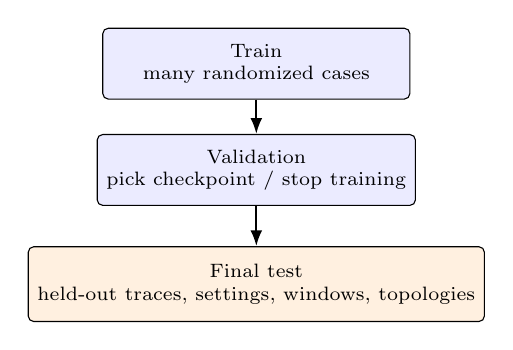
\begin{tikzpicture}[
          x=1cm, y=1cm,
          phase/.style={draw, rounded corners=2pt, minimum width=3.9cm, minimum height=0.9cm, align=center, font=\scriptsize, fill=blue!8},
          result/.style={draw, rounded corners=2pt, minimum width=3.9cm, minimum height=0.95cm, align=center, font=\scriptsize, fill=orange!12},
          arr/.style={-{Latex[length=2mm]}, thick}
      ]
        \node[phase] (train) at (2.2,2.8) {Train\\many randomized cases};
        \node[phase] (val) at (2.2,1.45) {Validation\\pick checkpoint / stop training};
        \node[result] (test) at (2.2,0.0) {Final test\\held-out traces, settings, windows, topologies};
        \draw[arr] (train) -- (val);
        \draw[arr] (val) -- (test);
      \end{tikzpicture}
    \column{0.48\textwidth}
      \begin{itemize}
        \item During training, we \textbf{intentionally vary} the environment so the policy learns a rule, not one instance.
        \item Validation is the tuning loop: it decides whether learning is improving.
        \item Final test is a firewall: those traces and settings stay untouched until the end.
        \item Repeated random pod mappings in test give a distribution, not one lucky number.
      \end{itemize}

      \vspace{0.4em}
      {\scriptsize This is the evaluation discipline we want the audience to trust.}
  \end{columns}

  \vspace{0.2em}
  {\tiny Current code already supports repeated pod remapping in \texttt{evaluate.py}; the broader split is the proposed experimental protocol.}
\end{frame}

\begin{frame}{Exact Technical Implementation of This Split}
  \begin{columns}[T,onlytextwidth]
    \column{0.54\textwidth}
      \scriptsize
      \begin{tabular}{p{0.27\linewidth}p{0.65\linewidth}}
        \toprule
        \textbf{Component} & \textbf{Implementation change} \\
        \midrule
        Train config & Replace single-trace args with a train manifest: traces, topology IDs, CXL fractions, and time windows. \\
        Env creation & In \texttt{\_make\_env()}, sample one case from that manifest at episode reset. \\
        Validation & Keep a separate fixed validation manifest and point \texttt{EvalCallback} only to it. \\
        Best model & Save checkpoints by validation reward, then freeze the best one for test. \\
        Final test & Make \texttt{evaluate.py} iterate over a held-out test manifest with the current repeated pod remaps. \\
        Reporting & Report mean / min / max / std per case and then aggregate across cases. \\
        \bottomrule
      \end{tabular}
    \column{0.46\textwidth}
      \begin{itemize}
        \item \textbf{Minimal code shape:}
      \end{itemize}
      \begin{block}{Suggested flow}
        \scriptsize
        train.py reads a train manifest and randomizes episodes from it.\\[0.3em]
        A fixed validation manifest selects the best checkpoint.\\[0.3em]
        evaluate.py runs that checkpoint on a held-out test manifest with 50 pod remaps per case.
      \end{block}
      \begin{itemize}
        \item This keeps the current code structure, but makes the split explicit and reproducible.
        \item It also gives a clean answer when asked: ``what exactly was seen during training?''
      \end{itemize}
  \end{columns}

  \vspace{0.2em}
  {\tiny Based on the current \texttt{train.py} / \texttt{evaluate.py} structure, with proposed extensions for manifests and held-out suites.}
\end{frame}

\begin{frame}{Training Budget Is Part of the Systems Story}
  \begin{columns}[T,onlytextwidth]
    \column{0.52\textwidth}
      \centering
      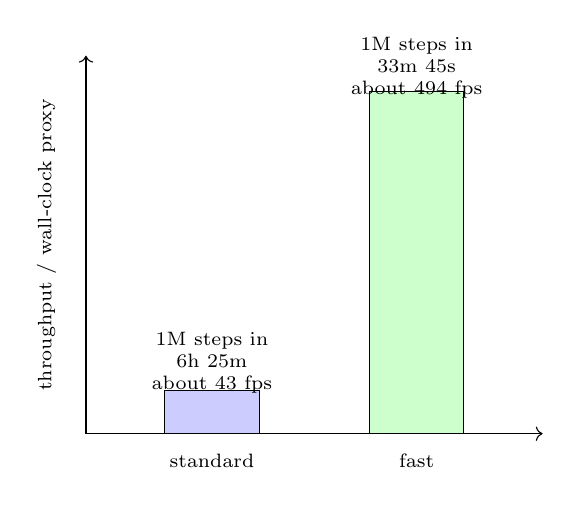
\begin{tikzpicture}[
          x=1cm, y=1cm,
          lbl/.style={font=\scriptsize},
          barA/.style={draw, fill=blue!20},
          barB/.style={draw, fill=green!20}
      ]
        \draw[->] (0,0) -- (0,4.8);
        \draw[->] (0,0) -- (5.8,0);
        \node[lbl, rotate=90] at (-0.5,2.4) {throughput / wall-clock proxy};
        \node[lbl] at (1.6,-0.35) {standard};
        \node[lbl] at (4.2,-0.35) {fast};
        \draw[barA] (1.0,0) rectangle (2.2,0.55);
        \draw[barB] (3.6,0) rectangle (4.8,4.35);
        \node[lbl, align=center] at (1.6,0.9) {1M steps in\\6h 25m\\about 43 fps};
        \node[lbl, align=center] at (4.2,4.65) {1M steps in\\33m 45s\\about 494 fps};
      \end{tikzpicture}
    \column{0.48\textwidth}
      \begin{itemize}
        \item Current logs show that training configuration changes wall-clock cost by an order of magnitude.
        \item Standard 1M-step SAC run: about \textbf{6h 25m}; fast 1M-step SAC run: about \textbf{33m 45s}.
        \item Current SAC training also does limited optimization work relative to collected experience.
        \item In \texttt{--fast}, the code uses \texttt{train\_freq=16} and \texttt{gradient\_steps=1}: one gradient update for every 16 env steps.
        \item That likely improves throughput, but it may also leave the policy under-optimized and hurt generalization.
      \end{itemize}

      \vspace{0.4em}
      {\scriptsize Timing comes from current training logs; update-frequency details come directly from current \texttt{train.py}.}
  \end{columns}
\end{frame}

\section{Model Choice}

% Sources:
% - context/cluade-convo-summary.md §9
% - context/rl_memory_pooling_roadmap_v2.md §§6, 7, 8
\begin{frame}{Off-Policy vs On-Policy vs Online RL}
  \scriptsize
  \begin{tabular}{p{0.16\linewidth}p{0.22\linewidth}p{0.23\linewidth}p{0.26\linewidth}}
    \toprule
    \textbf{Setting} & \textbf{What data it learns from} & \textbf{Main strength} & \textbf{Main risk for Octopus} \\
    \midrule
    Off-policy & old + new experience via replay & sample efficient & mixes regimes; can destabilize on drifting traces \\
    On-policy & only fresh rollouts from the current policy & cleaner updates & needs many more environment steps \\
    Online RL & keeps updating after deployment starts & adapts to real drift & can forget old regimes or destabilize behavior \\
    \bottomrule
  \end{tabular}

  \vspace{0.35em}
  \begin{columns}[T,onlytextwidth]
    \column{0.52\textwidth}
      \begin{block}{How this maps to our methods}
        \scriptsize
        SAC = off-policy offline baseline\\
        PPO = on-policy offline learnability test\\
        LCPO = online adaptation with forgetting control
      \end{block}
    \column{0.48\textwidth}
      \scriptsize
      \begin{itemize}
        \item The distinction is about \textbf{where updates come from}, not just about algorithm names.
        \item Our roadmap is: first solve the offline task, then decide whether online adaptation is needed.
      \end{itemize}
  \end{columns}
\end{frame}

\begin{frame}{SAC: What It Is and Why We Started Here}
  \begin{columns}[T,onlytextwidth]
    \column{0.48\textwidth}
      \begin{block}{Core idea}
        \scriptsize
        Soft Actor-Critic is an \textbf{off-policy} method for continuous actions.\\[0.2em]
        It keeps a replay buffer, reuses old experience, and optimizes both reward and exploration.
      \end{block}

      \begin{block}{Useful equation}
        \scriptsize
        \begin{equation*}
        J_{\pi}
        =
        \mathbb{E}\bigl[Q(s,a) - \alpha \log \pi(a|s)\bigr]
        \end{equation*}
        \begin{equation*}
        y
        =
        r + \gamma\bigl(Q_{\mathrm{targ}}(s',a') - \alpha \log \pi(a'|s')\bigr)
        \end{equation*}
        \scriptsize
        High-value actions are preferred, but the entropy term keeps exploration alive.
      \end{block}
    \column{0.52\textwidth}
      \scriptsize
      \begin{itemize}
        \item \textbf{Fit for Octopus:} our action is a continuous allocation vector.
        \item \textbf{Why start here:} replay makes SAC sample efficient offline.
        \item \textbf{Key risk:} replay mixes old and new regimes, which can destabilize learning on non-stationary traces.
        \item \textbf{Question it answers:} can an off-policy continuous controller learn the allocator at all?
      \end{itemize}
  \end{columns}

  \vspace{0.2em}
  {\tiny SAC: Haarnoja et al., \href{https://arxiv.org/abs/1801.01290}{arXiv:1801.01290}}
\end{frame}

\begin{frame}{PPO: Simpler Policy-Gradient Baseline}
  \begin{columns}[T,onlytextwidth]
    \column{0.50\textwidth}
      \begin{block}{Core idea}
        \scriptsize
        Proximal Policy Optimization is an \textbf{on-policy} method.\\[0.2em]
        It collects a fresh rollout, computes advantages, and then updates the policy while explicitly limiting how far the policy can move in one step.
      \end{block}

      \begin{block}{Useful equation}
        \scriptsize
        \begin{equation*}
        L^{\mathrm{clip}}
        =
        \mathbb{E}\Bigl[
        \min\bigl(
        r_t A_t,\;
        \mathrm{clip}(r_t,1-\epsilon,1+\epsilon)A_t
        \bigr)
        \Bigr]
        \end{equation*}
        \begin{equation*}
        r_t = \frac{\pi_{\theta}(a_t|s_t)}{\pi_{\theta_{\mathrm{old}}}(a_t|s_t)}
        \end{equation*}
        \scriptsize
        Take a policy-gradient step, but clip updates so the policy cannot jump too far.
      \end{block}
    \column{0.50\textwidth}
      \scriptsize
      \begin{itemize}
        \item \textbf{Why it matters:} PPO removes replay-buffer effects and uses fresh rollouts only.
        \item \textbf{Why systems people like it:} cleaner updates make debugging easier.
        \item \textbf{Trade-off:} usually more stable than SAC, but less sample efficient.
        \item \textbf{Question it answers:} if PPO still fails, the bottleneck is probably state / reward / observability, not just SAC instability.
      \end{itemize}
  \end{columns}

  \vspace{0.2em}
  {\tiny PPO: Schulman et al., \href{https://arxiv.org/abs/1707.06347}{arXiv:1707.06347}}
\end{frame}

\begin{frame}{LCPO: Online Adaptation Without Forgetting}
  \begin{columns}[T,onlytextwidth]
    \column{0.50\textwidth}
      \begin{block}{Core idea}
        \scriptsize
        LCPO is an \textbf{on-policy online adaptation} method for non-stationary environments.\\[0.2em]
        It updates on recent data, but constrains the new policy so it does not drift too much on older, different contexts.
      \end{block}

      \begin{block}{Useful equation}
        \scriptsize
        \begin{equation*}
        \max_{\theta}\;
        L_{\mathrm{recent}}(\theta; B_r) + \lambda H(\pi_\theta)
        \end{equation*}
        \begin{equation*}
        \text{s.t.}\quad
        D_{\mathrm{KL}}\!\bigl(
        \pi_{\theta_{\mathrm{old}}} \,\|\, \pi_{\theta};
        S_c
        \bigr)
        \le c_{\mathrm{anchor}}
        \end{equation*}
        \scriptsize
        Improve on the current workload, but do not drift too far on anchor samples from old contexts.
      \end{block}
    \column{0.50\textwidth}
      \scriptsize
      \begin{itemize}
        \item \textbf{Anchor set:} keep a few old contexts, like morning-load samples while adapting to evening load.
        \item \textbf{Why it matters:} deployment traffic is non-stationary, so online learning can forget earlier regimes.
        \item \textbf{What it adds beyond PPO:} forgetting resistance, not better base-task learning.
        \item \textbf{Question it answers:} once the allocator works, can it adapt online without breaking old behavior?
      \end{itemize}
  \end{columns}

  \vspace{0.2em}
  {\tiny LCPO: Hamadanian et al., \href{https://lcpo.csail.mit.edu/content/lcpo-iclr.pdf}{ICLR paper}}
\end{frame}

\begin{frame}{Which Algorithm Solves Which Problem?}
  \begin{columns}[T,onlytextwidth]
    \column{0.33\textwidth}
      \begin{block}{SAC}
        \begin{itemize}
          \item continuous allocation vector
          \item sample efficient
          \item risk: off-policy instability
          \item role: current baseline
        \end{itemize}
      \end{block}
    \column{0.33\textwidth}
      \begin{block}{PPO}
        \begin{itemize}
          \item same action space
          \item simpler updates
          \item risk: less sample efficient
          \item role: test base learnability
        \end{itemize}
      \end{block}
    \column{0.33\textwidth}
      \begin{block}{LCPO}
        \begin{itemize}
          \item online non-stationary learning
          \item forgetting resistance
          \item risk: more complexity
          \item role: deployment-time method
        \end{itemize}
      \end{block}
  \end{columns}

  \vspace{0.4em}
  \begin{itemize}
    \item This deck is not arguing ``LCPO now''.
    \item It is arguing ``fix the base task first, then move to deployment-time methods''.
  \end{itemize}

  \vspace{0.2em}
  {\tiny SAC: Haarnoja et al., \href{https://arxiv.org/abs/1801.01290}{arXiv:1801.01290} \hspace{1em}
  PPO: Schulman et al., \href{https://arxiv.org/abs/1707.06347}{arXiv:1707.06347} \hspace{1em}
  LCPO: Hamadanian et al., \href{https://lcpo.csail.mit.edu/content/lcpo-iclr.pdf}{ICLR paper}}
\end{frame}

\begin{frame}{Recommended Order: SAC, Then PPO, Then LCPO}
  \centering
  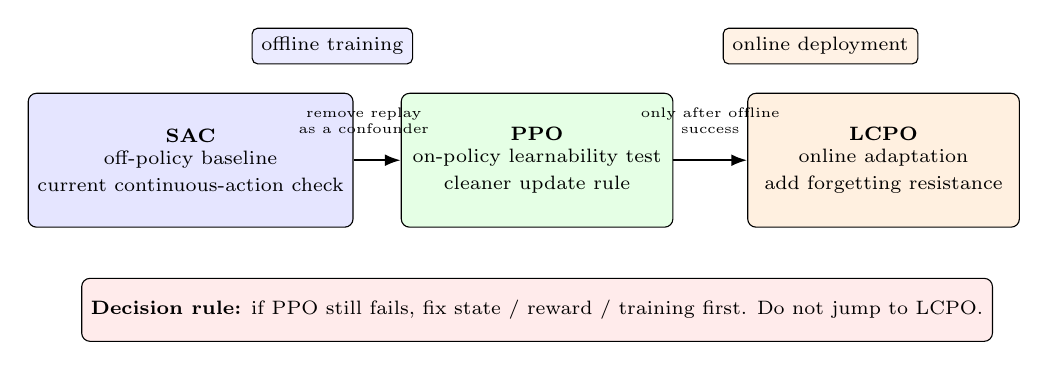
\begin{tikzpicture}[
      x=1cm, y=1cm,
      stage/.style={draw, rounded corners=3pt, minimum width=3.45cm, minimum height=1.7cm, align=center, font=\scriptsize},
      tag/.style={draw, rounded corners=2pt, minimum width=2.0cm, minimum height=0.45cm, align=center, font=\scriptsize, fill=black!6},
      note/.style={draw, rounded corners=3pt, minimum width=8.6cm, minimum height=0.8cm, align=center, font=\scriptsize, fill=red!8},
      arr/.style={-{Latex[length=2mm]}, thick}
  ]
    \node[tag, fill=blue!8] at (4.0,3.1) {offline training};
    \node[tag, fill=orange!10] at (10.2,3.1) {online deployment};

    \node[stage, fill=blue!10] (sac) at (2.2,1.65) {
      \textbf{SAC}\\
      off-policy baseline\\[0.2em]
      current continuous-action check
    };
    \node[stage, fill=green!10] (ppo) at (6.6,1.65) {
      \textbf{PPO}\\
      on-policy learnability test\\[0.2em]
      cleaner update rule
    };
    \node[stage, fill=orange!12] (lcpo) at (11.0,1.65) {
      \textbf{LCPO}\\
      online adaptation\\[0.2em]
      add forgetting resistance
    };
    \draw[arr] (sac) -- (ppo);
    \draw[arr] (ppo) -- (lcpo);
    \node[font=\tiny, align=center] at (4.4,2.15) {remove replay\\as a confounder};
    \node[font=\tiny, align=center] at (8.8,2.15) {only after offline\\success};

    \node[note] at (6.6,-0.25) {\textbf{Decision rule:} if PPO still fails, fix state / reward / training first. Do not jump to LCPO.};
  \end{tikzpicture}
\end{frame}

\section{Results and Evaluation}

% Sources:
% - octopus-allocation/scripts/plot_demand.py
% - context/cluade-convo-summary.md §4.4-4.5
\begin{frame}{Results We Already Have}
  \begin{columns}[T,onlytextwidth]
    \column{0.58\textwidth}
      \figorplaceholder{../octopus-allocation/docs/overview/v1/figs/demand_overview.pdf}{0.66\textheight}
    \column{0.42\textwidth}
      \begin{block}{Already supported}
        \begin{itemize}
          \item 10-datacenter trace evidence with clear diurnal structure
          \item cluster peak-to-mean ratio around 1.13--1.26x
          \item break-even at about 3\% savings
          \item prior Octopus result of about 16\% greedy savings on Acadia-96
        \end{itemize}
      \end{block}

      \vspace{0.3em}
      {\scriptsize This slide combines current files in the repo with older project evidence that should be clearly labeled as such.}
  \end{columns}
\end{frame}

\begin{frame}{Current Measured Limitation: Load Collapse}
  \begin{columns}[T,onlytextwidth]
    \column{0.46\textwidth}
      \centering
      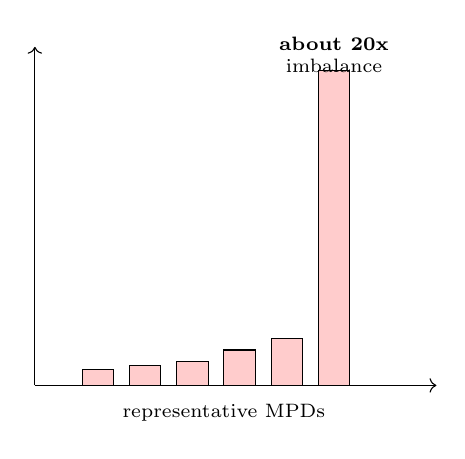
\begin{tikzpicture}[
          x=1cm, y=1cm,
          bar/.style={draw, fill=red!20},
          lbl/.style={font=\scriptsize}
      ]
        \draw[->] (0,0) -- (0,4.3);
        \draw[->] (0,0) -- (5.1,0);
        \draw[bar] (0.6,0) rectangle (1.0,0.2);
        \draw[bar] (1.2,0) rectangle (1.6,0.25);
        \draw[bar] (1.8,0) rectangle (2.2,0.3);
        \draw[bar] (2.4,0) rectangle (2.8,0.45);
        \draw[bar] (3.0,0) rectangle (3.4,0.6);
        \draw[bar] (3.6,0) rectangle (4.0,4.0);
        \node[lbl, align=center] at (3.8,4.2) {\textbf{about 20x}\\imbalance};
        \node[lbl] at (2.4,-0.35) {representative MPDs};
      \end{tikzpicture}
    \column{0.54\textwidth}
      \begin{itemize}
        \item The most concrete current failure signal is \textbf{about 20x max/min MPD imbalance}.
        \item For a systems audience, this is easier to reason about than an RL loss curve.
        \item It says the policy is not yet acting like a load balancer.
        \item This is the slide that justifies the state and reward redesign.
      \end{itemize}
  \end{columns}
\end{frame}

\begin{frame}{What Current Training Logs Tell Us}
  \begin{columns}[T,onlytextwidth]
    \column{0.52\textwidth}
      \begin{block}{Current-code measurements}
        \begin{itemize}
          \item Standard SAC, 1M steps: final eval reward about \textbf{-3.17}.
          \item Fast SAC, 1M steps: final eval reward about \textbf{-2.71}.
          \item Eval reward is still noisy throughout training.
          \item Current code does \emph{not} log pooling savings during training.
        \end{itemize}
      \end{block}
    \column{0.48\textwidth}
      \centering
      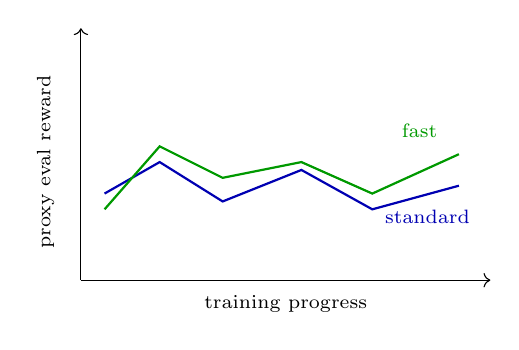
\begin{tikzpicture}[
          x=1cm, y=1cm,
          lbl/.style={font=\scriptsize},
          lineA/.style={thick, blue!70!black},
          lineB/.style={thick, green!60!black}
      ]
        \draw[->] (0,0) -- (0,3.2);
        \draw[->] (0,0) -- (5.2,0);
        \node[lbl, rotate=90] at (-0.45,1.5) {proxy eval reward};
        \node[lbl] at (2.6,-0.3) {training progress};
        \draw[lineA] (0.3,1.1) -- (1.0,1.5) -- (1.8,1.0) -- (2.8,1.4) -- (3.7,0.9) -- (4.8,1.2);
        \draw[lineB] (0.3,0.9) -- (1.0,1.7) -- (1.8,1.3) -- (2.8,1.5) -- (3.7,1.1) -- (4.8,1.6);
        \node[lbl, blue!70!black] at (4.4,0.8) {standard};
        \node[lbl, green!60!black] at (4.3,1.9) {fast};
      \end{tikzpicture}
  \end{columns}

  \vspace{0.4em}
  {\scriptsize Useful conclusion: current proxy rewards show progress but are still not the systems metric we actually care about.}
\end{frame}

\begin{frame}{What the Current Code Path Still Does Not Give Us}
  \begin{itemize}
    \item No pooling-savings curve over training time
    \item No saved greedy-vs-RL comparison table in the new scripted pipeline
    \item No per-MPD load timeline plot produced automatically from the current run
    \item No curriculum stages or train/validation/test suite yet
  \end{itemize}

  \vspace{0.5em}
  \begin{block}{Why this matters}
    For a systems audience, the next milestone is not just ``better reward'' but ``better observability of the allocator''.
  \end{block}
\end{frame}

\begin{frame}{Results Dashboard To Add Next}
  \scriptsize
  \begin{tabular}{p{0.18\linewidth}p{0.25\linewidth}p{0.23\linewidth}p{0.25\linewidth}}
    \toprule
    \textbf{Experiment} & \textbf{What we vary} & \textbf{What we report} & \textbf{What it tells us} \\
    \midrule
    State ablation &
    load-only vs +pressure vs +temporal features &
    savings, MPD imbalance, oversubscribed MPDs &
    whether missing observability causes load collapse \\
    Reward ablation &
    peak-only vs peak+variance vs full reward &
    savings, over-cap violations, reward stability &
    whether the reward matches the systems objective \\
    Training ablation &
    1M vs 10M vs 50M+, with and without curriculum / randomization &
    validation savings, held-out savings, wall-clock &
    whether we are under-training or mis-specifying the task \\
    Algorithm comparison &
    SAC vs PPO offline; LCPO only in online drift setting &
    held-out performance, forgetting, update cost &
    whether a new learner helps, or the base task still needs fixing \\
    \bottomrule
  \end{tabular}

  \vspace{0.35em}
  \begin{block}{Minimum dashboard plots}
    \scriptsize
    Greedy-vs-RL savings table, per-MPD load timeline, oversubscribed-MPD count, and train / validation / test curves on held-out cases.
  \end{block}
\end{frame}

\begin{frame}{Expected Outcomes}
  \begin{itemize}
    \item Better state and reward should remove the current load-collapse behavior.
    \item Better training should improve offline generalization before any online method is introduced.
    \item PPO should be the clean baseline for asking whether the base task is learnable.
    \item LCPO should matter only once PPO is already competent and online drift becomes the bottleneck.
  \end{itemize}
\end{frame}

\begin{frame}{Takeaways}
  \begin{itemize}
    \item The systems opportunity is real: real traces show headroom, and prior Octopus results already clear break-even comfortably.
    \item The current RL issue is not ``pick a fancier algorithm''; it is that the present task formulation is too hard to learn well.
    \item The first fixes are better state, better reward, better observability, and more disciplined training.
    \item The right comparison order is SAC, then PPO, then LCPO.
    \item Once we have those pieces, we can slim this deck down into a shorter talk very easily.
  \end{itemize}
\end{frame}

\end{document}
